%%%%%%%%%%%%%%%%%%%%%%%%%%%%%%%%%%%%%%%%%%%%%%%%%%%
%
%  New template code for TAMU Theses and Dissertations starting Fall 2012.  
%  For more info about this template or the 
%  TAMU LaTeX User's Group, see http://www.howdy.me/.
%
%  Author: Wendy Lynn Turner 
%	 Version 1.0 
%  Last updated 8/5/2012
%
%%%%%%%%%%%%%%%%%%%%%%%%%%%%%%%%%%%%%%%%%%%%%%%%%%%

%%%%%%%%%%%%%%%%%%%%%%%%%%%%%%%%%%%%%%%%%%%%%%%%%%%%%%%%%%%%%%%%%%%%%%
%%                           APPENDIX B
%%%%%%%%%%%%%%%%%%%%%%%%%%%%%%%%%%%%%%%%%%%%%%%%%%%%%%%%%%%%%%%%%%%%%

\chapter{\texorpdfstring{\MakeUppercase{ZONE LOADS FOR NCTM}}{Zone Loads
for NCTM}}

\section{Estimated Zone Loads for NCTM}

This portion of the appendix plots all the zone loads for the terminal
units at NCTM. 

\newcommand{\zoneLoadAppendixPlotsCaption}[1]{Zone load for #1 during
the year 2016.}

\section{Terminal Units of AHU-2-1}
%Plots/04/2017-06-27-0830-BtuhrvsOADryBulbTemperatureNOAAF.tex
\begin{figure}
    \centering
    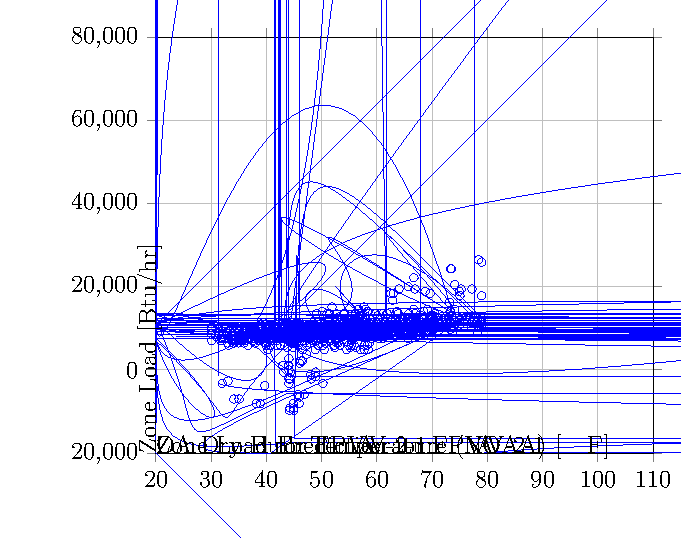
\includegraphics{Plots/04/2017-06-27-0830-BtuhrvsOADryBulbTemperatureNOAAF.pdf}
    \caption{\zoneLoadAppendixPlotsCaption{FPVAV-2-1}}
    \label{fig:2017-06-27-0830-BtuhrvsOADryBulbTemperatureNOAAF}
\end{figure}

\begin{figure}
    \centering
    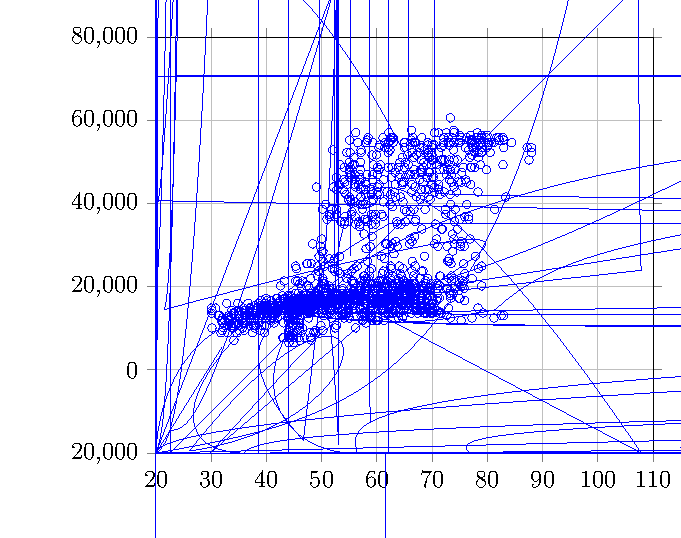
\includegraphics{Plots/05/2017-06-27-1012-BtuhrvsOADryBulbTemperatureNOAAF.pdf}
    \caption{\zoneLoadAppendixPlotsCaption{FPVAV-2-2}}
    \label{fig:2017-06-27-1012-BtuhrvsOADryBulbTemperatureNOAAF}
\end{figure}

\begin{figure}
\centering
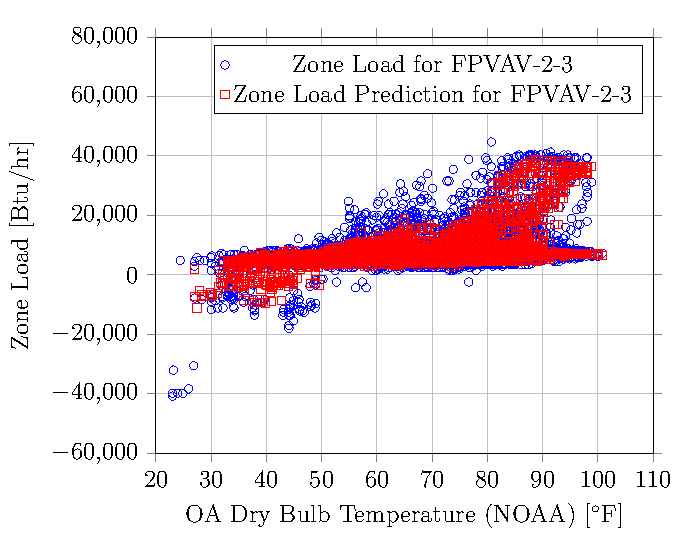
\includegraphics{Plots/06/2017-06-27-1018-BtuhrvsOADryBulbTemperatureNOAAF.pdf}
\caption{\zoneLoadAppendixPlotsCaption{FPVAV-2-3} Notice that the lower
bound of the y-axis is different than the other plots. }
\label{fig:2017-06-27-1018-BtuhrvsOADryBulbTemperatureNOAAF}
\end{figure}


\clearpage

\section{Terminal Units of AHU-2-2}

\begin{figure}
\centering
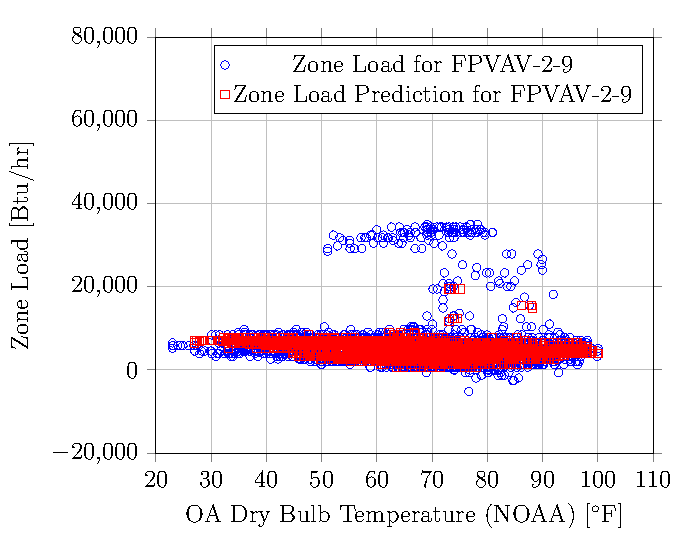
\includegraphics{Plots/07/2017-06-27-1026-BtuhrvsOADryBulbTemperatureNOAAF.pdf}
\caption{\zoneLoadAppendixPlotsCaption{FPVAV-2-9}}
\label{fig:2017-06-27-1026-BtuhrvsOADryBulbTemperatureNOAAF}
\end{figure}

\begin{figure}
\centering
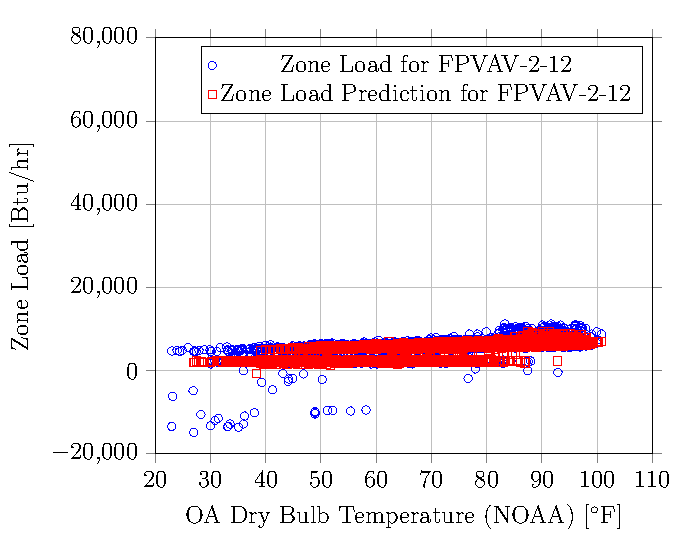
\includegraphics{Plots/08/2017-06-27-1058-BtuhrvsOADryBulbTemperatureNOAAF.pdf}
\caption{\zoneLoadAppendixPlotsCaption{FPVAV-2-12}}
\label{fig:2017-06-27-1058-BtuhrvsOADryBulbTemperatureNOAAF}
\end{figure}


\begin{figure}
\centering
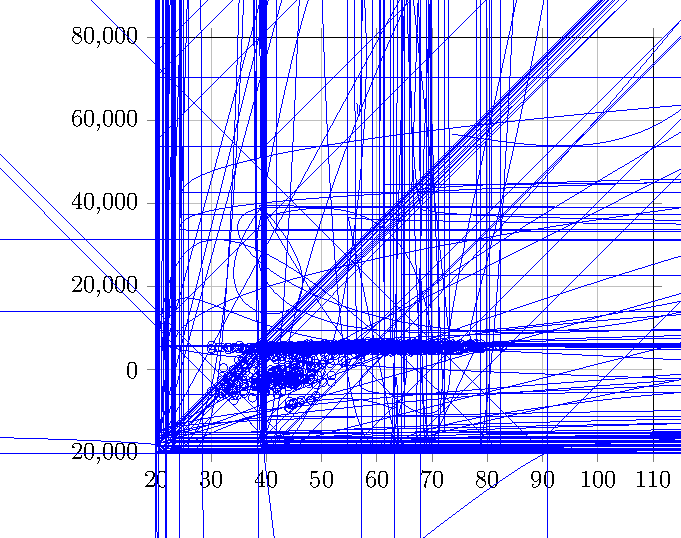
\includegraphics{Plots/09/2017-06-27-1124-BtuhrvsOADryBulbTemperatureNOAAF.pdf}
\caption{\zoneLoadAppendixPlotsCaption{FPVAV-2-13}}
\label{fig:2017-06-27-1124-BtuhrvsOADryBulbTemperatureNOAAF}
\end{figure}

\begin{figure}
\centering
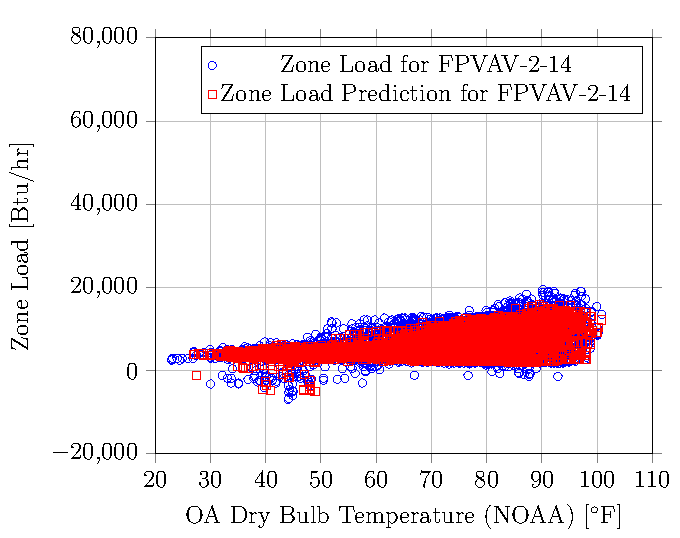
\includegraphics{Plots/10/2017-06-27-1131-BtuhrvsOADryBulbTemperatureNOAAF.pdf}
\caption{\zoneLoadAppendixPlotsCaption{FPVAV-2-14}}
\label{fig:2017-06-27-1131-BtuhrvsOADryBulbTemperatureNOAAF}
\end{figure}

\begin{figure}
\centering
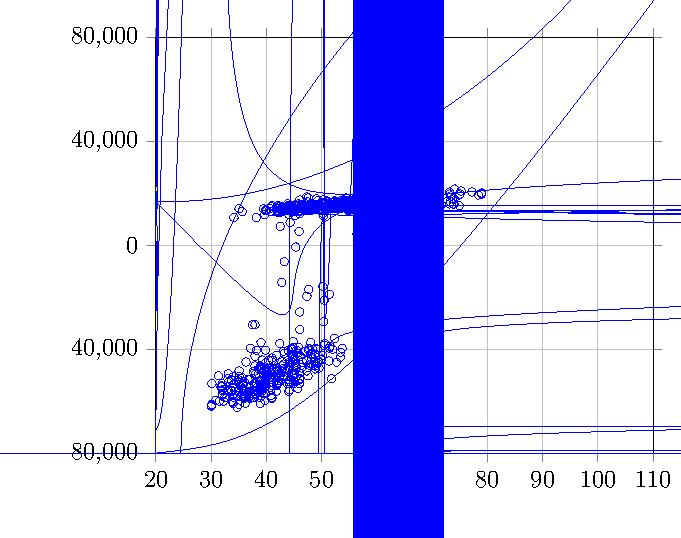
\includegraphics{Plots/11/2017-06-27-1135-BtuhrvsOADryBulbTemperatureNOAAF.pdf}
\caption{\zoneLoadAppendixPlotsCaption{FPVAV-2-15} Notice that the lower
bound of the y-axis is different than the other plots.}
\label{fig:2017-06-27-1135-BtuhrvsOADryBulbTemperatureNOAAF}
\end{figure}

\begin{figure}
\centering
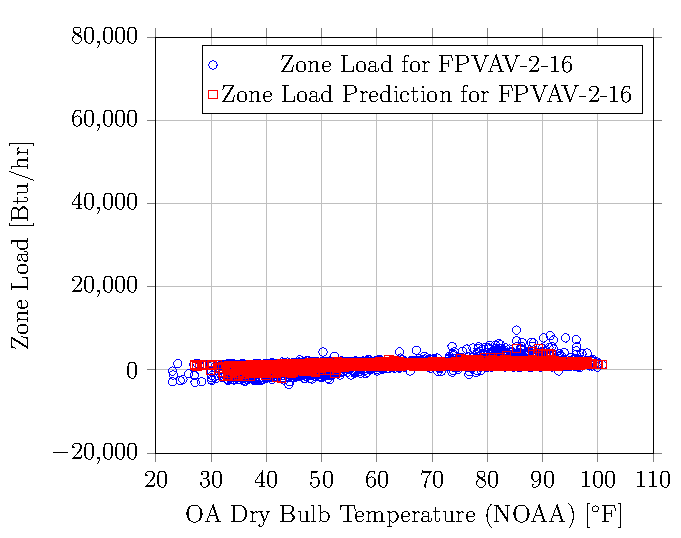
\includegraphics{Plots/12/2017-06-27-1138-BtuhrvsOADryBulbTemperatureNOAAF.pdf}
\caption{\zoneLoadAppendixPlotsCaption{FPVAV-2-16}}
\label{fig:2017-06-27-1138-BtuhrvsOADryBulbTemperatureNOAAF}
\end{figure}


\begin{figure}
    \centering
    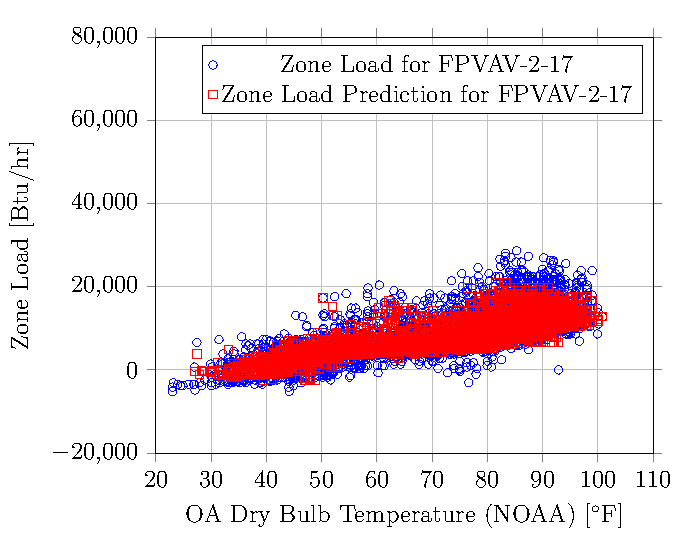
\includegraphics{Plots/13/2017-06-27-1141-BtuhrvsOADryBulbTemperatureNOAAF.pdf}
    \caption{\zoneLoadAppendixPlotsCaption{FPVAV-2-17}}
    \label{fig:2017-06-27-1141-BtuhrvsOADryBulbTemperatureNOAAF}
\end{figure}

\begin{figure}
\centering
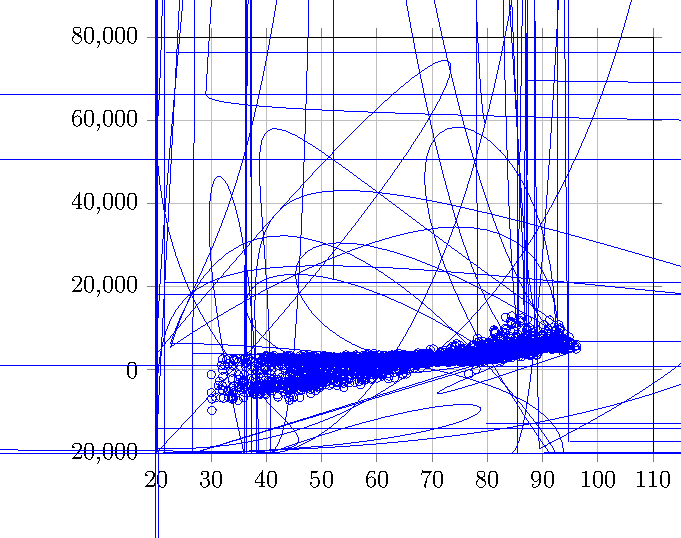
\includegraphics{Plots/14/2017-06-27-1145-BtuhrvsOADryBulbTemperatureNOAAF.pdf}
\caption{\zoneLoadAppendixPlotsCaption{FPVAV-2-18}}
\label{fig:2017-06-27-1145-BtuhrvsOADryBulbTemperatureNOAAF}
\end{figure}


\section{Terminal Units of AHU-2-3}

\begin{figure}
\centering
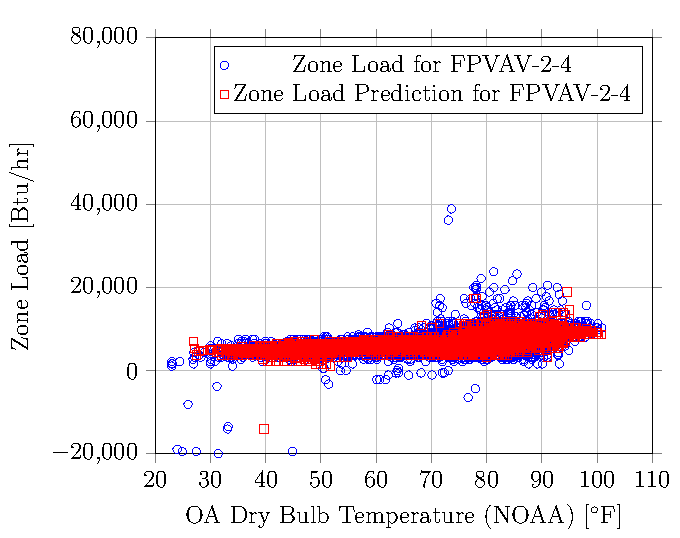
\includegraphics[]{Plots/15/2017-06-27-1319-BtuhrvsOADryBulbTemperatureNOAAF.pdf}
\caption{\zoneLoadAppendixPlotsCaption{FPVAV-2-4}}
\label{fig:2017-06-27-1319-BtuhrvsOADryBulbTemperatureNOAAF}
\end{figure}

\begin{figure}
\centering
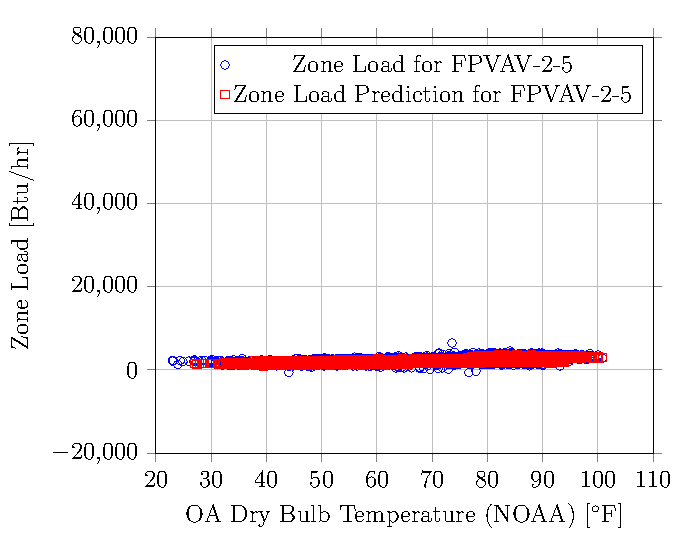
\includegraphics[]{Plots/16/2017-06-27-1322-BtuhrvsOADryBulbTemperatureNOAAF.pdf}
\caption{\zoneLoadAppendixPlotsCaption{FPVAV-2-5}}
\label{fig:2017-06-27-1322-BtuhrvsOADryBulbTemperatureNOAAF}
\end{figure}

\begin{figure}
\centering
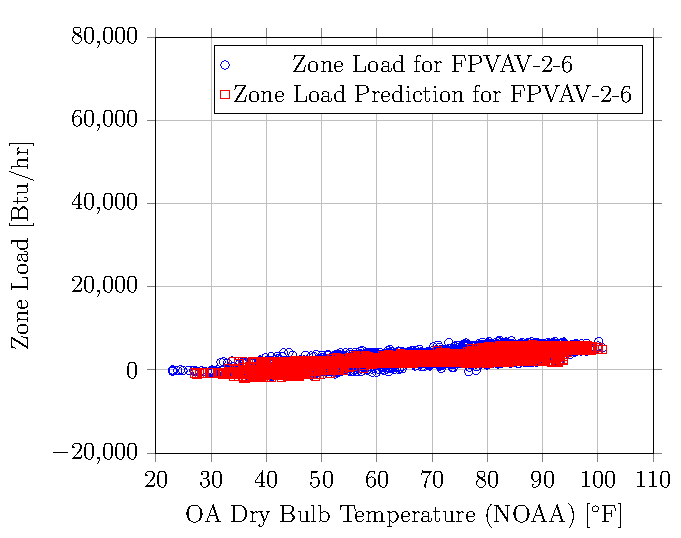
\includegraphics[]{Plots/17/2017-06-27-1325-BtuhrvsOADryBulbTemperatureNOAAF.pdf}
\caption{\zoneLoadAppendixPlotsCaption{FPVAV-2-6}}
\label{fig:2017-06-27-1325-BtuhrvsOADryBulbTemperatureNOAAF}
\end{figure}


\begin{figure}
\centering
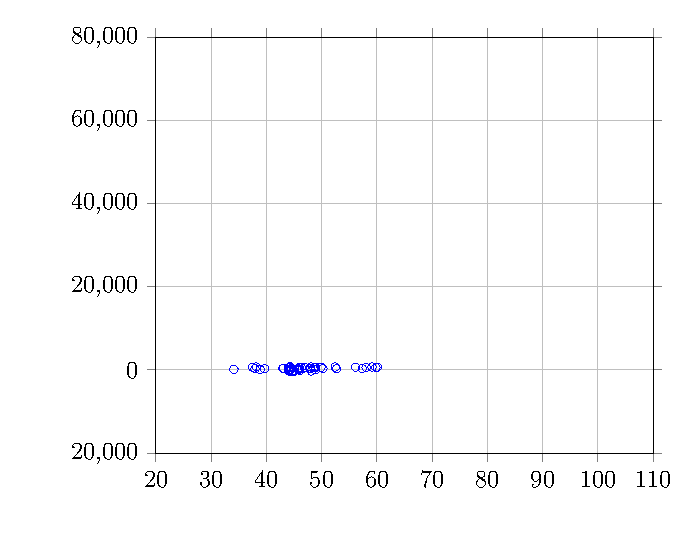
\includegraphics[]{Plots/18/2017-06-27-1328-BtuhrvsOADryBulbTemperatureNOAAF.pdf}
\caption{\zoneLoadAppendixPlotsCaption{FPVAV-2-7}}
\label{fig:2017-06-27-1328-BtuhrvsOADryBulbTemperatureNOAAF}
\end{figure}

\begin{figure}
\centering
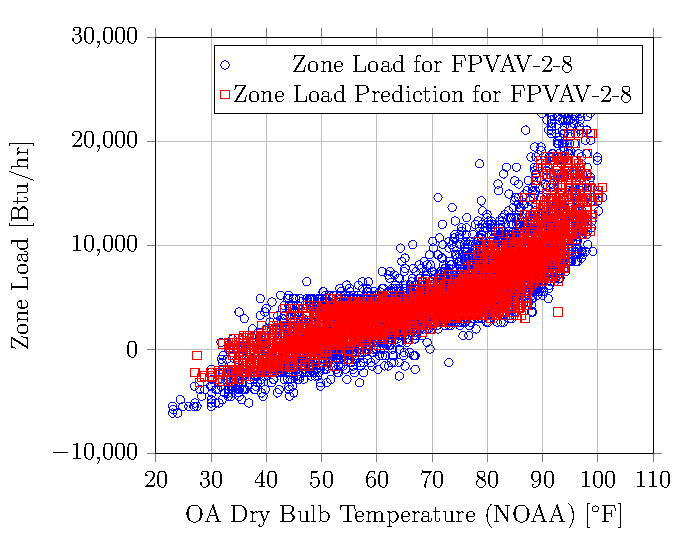
\includegraphics[]{Plots/19/2017-06-27-1330-BtuhrvsOADryBulbTemperatureNOAAF.pdf}
\caption{\zoneLoadAppendixPlotsCaption{FPVAV-2-8}}
\label{fig:2017-06-27-1330-BtuhrvsOADryBulbTemperatureNOAAF}
\end{figure}

\begin{figure}
\centering
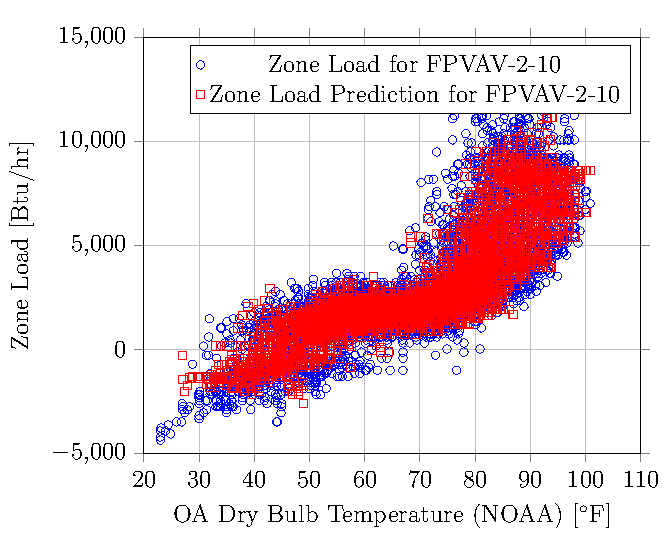
\includegraphics[]{Plots/20/2017-06-27-1332-BtuhrvsOADryBulbTemperatureNOAAF.pdf}
\caption{\zoneLoadAppendixPlotsCaption{FPVAV-2-10}}
\label{fig:2017-06-27-1332-BtuhrvsOADryBulbTemperatureNOAAF}
\end{figure}

\begin{figure}
\centering
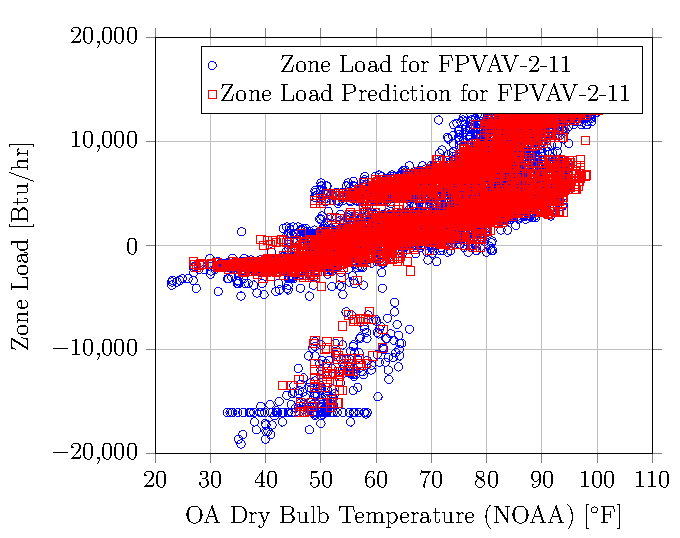
\includegraphics[]{Plots/21/2017-06-27-1334-BtuhrvsOADryBulbTemperatureNOAAF.pdf}
\caption{\zoneLoadAppendixPlotsCaption{FPVAV-2-11}}
\label{fig:2017-06-27-1334-BtuhrvsOADryBulbTemperatureNOAAF}
\end{figure}

\section{Terminal Units of AHU-1-2}

\begin{figure}
    \centering
    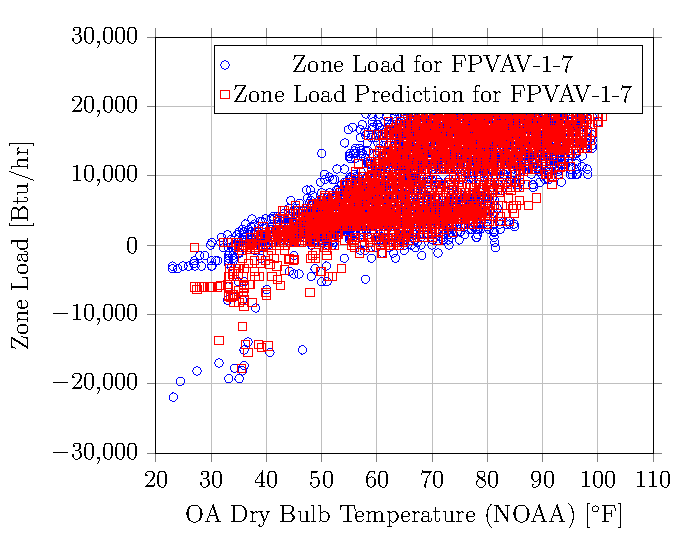
\includegraphics[]{Plots/22/2017-06-27-1343-BtuhrvsOADryBulbTemperatureNOAAF.pdf}
    \caption{\zoneLoadAppendixPlotsCaption{FPVAV-1-7}}
    \label{fig:2017-06-27-1343-BtuhrvsOADryBulbTemperatureNOAAF}
\end{figure}

\begin{figure}
\centering
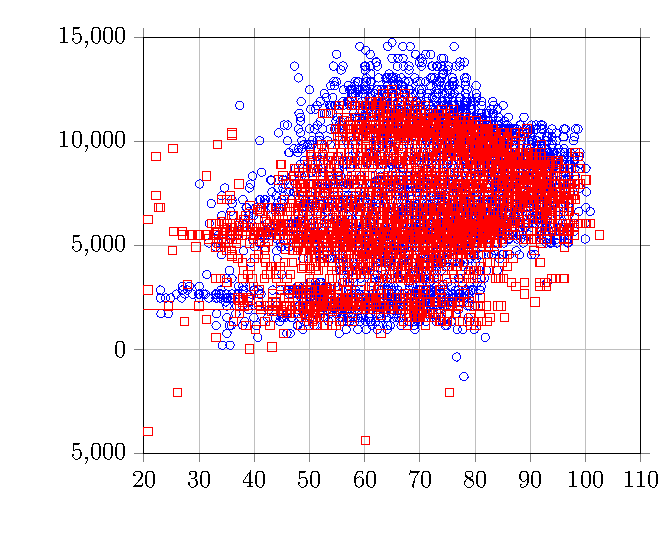
\includegraphics[]{Plots/23/2017-06-27-1346-BtuhrvsOADryBulbTemperatureNOAAF.pdf}
\caption{\zoneLoadAppendixPlotsCaption{FPVAV-1-8}}
\label{fig:2017-06-27-1346-BtuhrvsOADryBulbTemperatureNOAAF}
\end{figure}

\begin{figure}
\centering
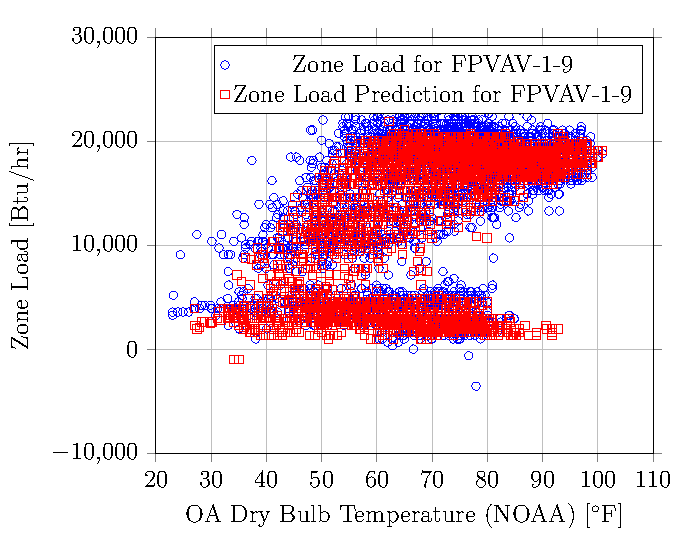
\includegraphics[]{Plots/24/2017-06-27-1348-BtuhrvsOADryBulbTemperatureNOAAF.pdf}
\caption{\zoneLoadAppendixPlotsCaption{FPVAV-1-9}}
\label{fig:2017-06-27-1348-BtuhrvsOADryBulbTemperatureNOAAF}
\end{figure}

\begin{figure}
\centering
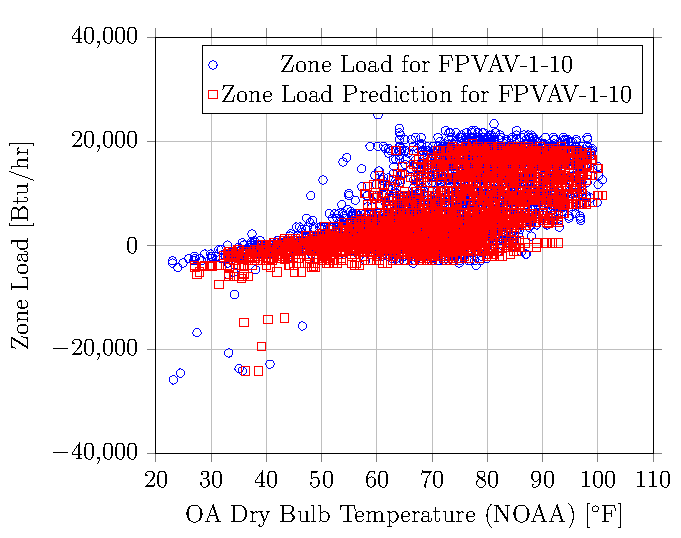
\includegraphics[]{Plots/25/2017-06-27-1353-BtuhrvsOADryBulbTemperatureNOAAF.pdf}
\caption{\zoneLoadAppendixPlotsCaption{FPVAV-1-10}}
\label{fig:2017-06-27-1353-BtuhrvsOADryBulbTemperatureNOAAF}
\end{figure}

\section{Terminal Units of AHU-1-3}

\begin{figure}
\centering
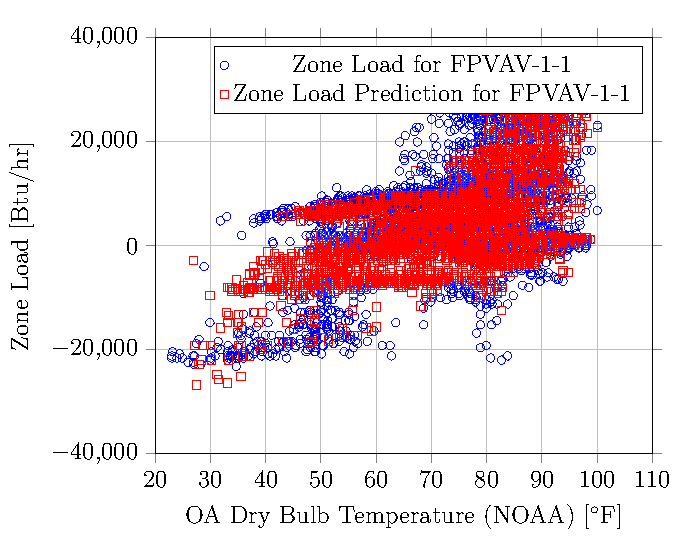
\includegraphics[]{Plots/26/2017-06-27-1355-BtuhrvsOADryBulbTemperatureNOAAF.pdf}
\caption{\zoneLoadAppendixPlotsCaption{FPVAV-1-1}}
\label{fig:2017-06-27-1355-BtuhrvsOADryBulbTemperatureNOAAF}
\end{figure}

\begin{figure}
\centering
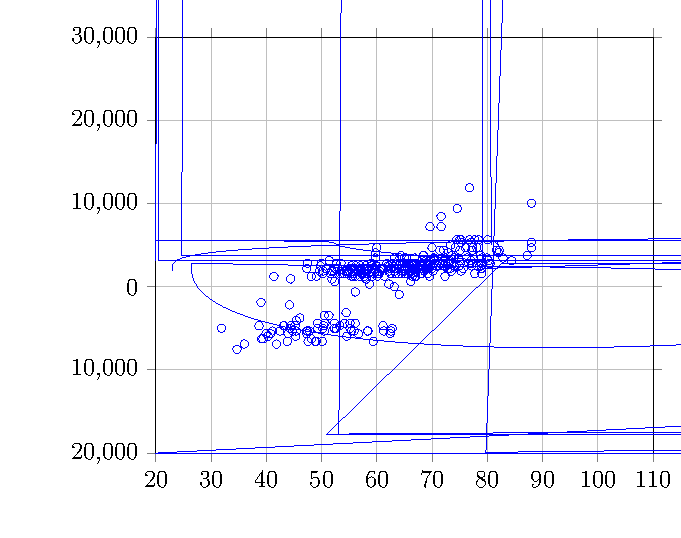
\includegraphics[]{Plots/27/2017-06-27-1356-BtuhrvsOADryBulbTemperatureNOAAF.pdf}
\caption{\zoneLoadAppendixPlotsCaption{FPVAV-1-2}}
\label{fig:2017-06-27-1356-BtuhrvsOADryBulbTemperatureNOAAF}
\end{figure}

\begin{figure}
\centering
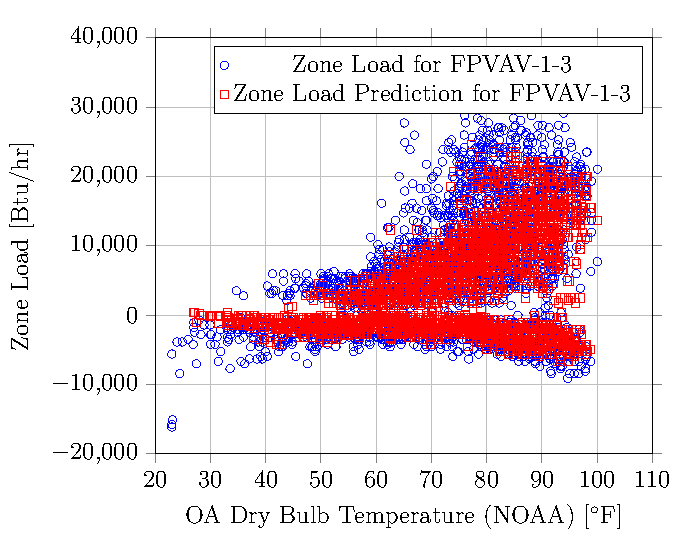
\includegraphics[]{Plots/28/2017-06-27-1357-BtuhrvsOADryBulbTemperatureNOAAF.pdf}
\caption{\zoneLoadAppendixPlotsCaption{FPVAV-1-3}}
\label{fig:2017-06-27-1357-BtuhrvsOADryBulbTemperatureNOAAF}
\end{figure}

\begin{figure}
\centering
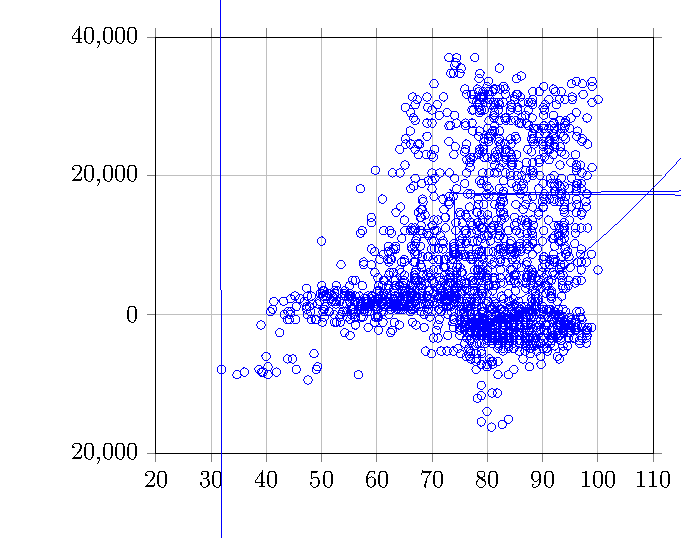
\includegraphics[]{Plots/29/2017-06-27-1358-BtuhrvsOADryBulbTemperatureNOAAF.pdf}
\caption{\zoneLoadAppendixPlotsCaption{FPVAV-1-4}}
\label{fig:2017-06-27-1358-BtuhrvsOADryBulbTemperatureNOAAF}
\end{figure}

\begin{figure}
\centering
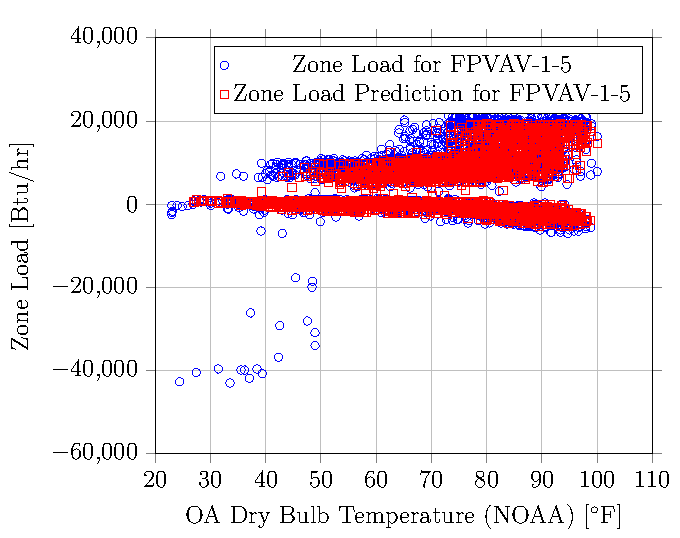
\includegraphics[]{Plots/30/2017-06-27-1359-BtuhrvsOADryBulbTemperatureNOAAF.pdf}
\caption{\zoneLoadAppendixPlotsCaption{FPVAV-1-5}}
\label{fig:2017-06-27-1359-BtuhrvsOADryBulbTemperatureNOAAF}
\end{figure}

\begin{figure}
\centering
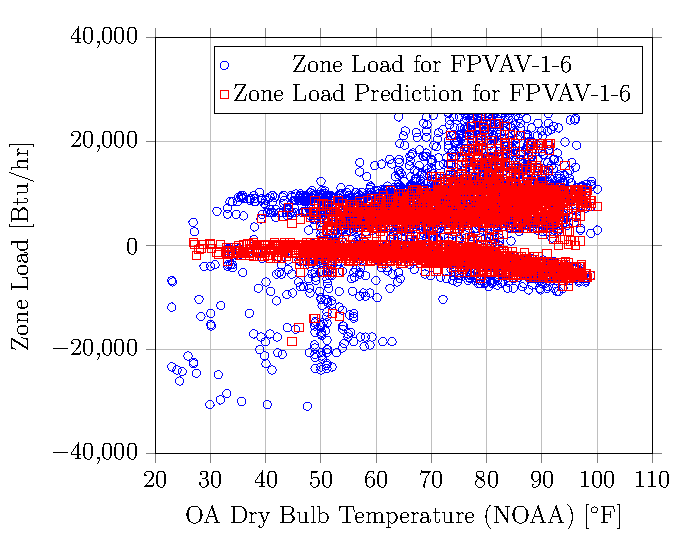
\includegraphics[]{Plots/31/2017-06-27-1400-BtuhrvsOADryBulbTemperatureNOAAF.pdf}
\caption{\zoneLoadAppendixPlotsCaption{FPVAV-1-6}}
\label{fig:2017-06-27-1401-BtuhrvsOADryBulbTemperatureNOAAF}
\end{figure}




\pagebreak{}
